\documentclass{beamer}
\usetheme{Madrid}
\usecolortheme{seahorse}

\title{Resultados del An\'alisis y Optimizaci\'on}
\author{}
\date{}

\begin{document}

\frame{\titlepage}

% --- Diapositiva 1: Introducci\'on a los Resultados ---
\begin{frame}{Resultados del An\'alisis}
\begin{block}{Objetivo}
Predecir la demanda semanal de 6 productos esenciales y optimizar las decisiones de compra bajo una restricci\'on presupuestaria.
\end{block}
\begin{itemize}
    \item Modelo: ARX (AutoRegresivo con variables ex\'ogenas)
    \item Horizonte de predicci\'on: 22 semanas
    \item Datos de entrenamiento: 56 semanas
\end{itemize}
\end{frame}

% --- Diapositiva 2: Predicci\'on de la demanda ---
\begin{frame}{ Predicci\'on de la demanda}
\begin{block}{Modelo ARX}
Se us\'o para estimar la demanda de pan, pollo, arroz, huevo, detergente y shampoo.
\end{block}
\begin{itemize}
    \item M\'etricas evaluadas: MAE, RMSE y MAPE
\end{itemize}
\vspace{0.3cm}
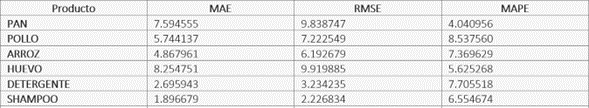
\includegraphics[width=0.75\textwidth]{error.png}
\end{frame}

% --- Diapositiva 3: Resultados visuales de la predicci\'on ---
\begin{frame}{Visualizaci\'on: Predicci\'on vs. Real}
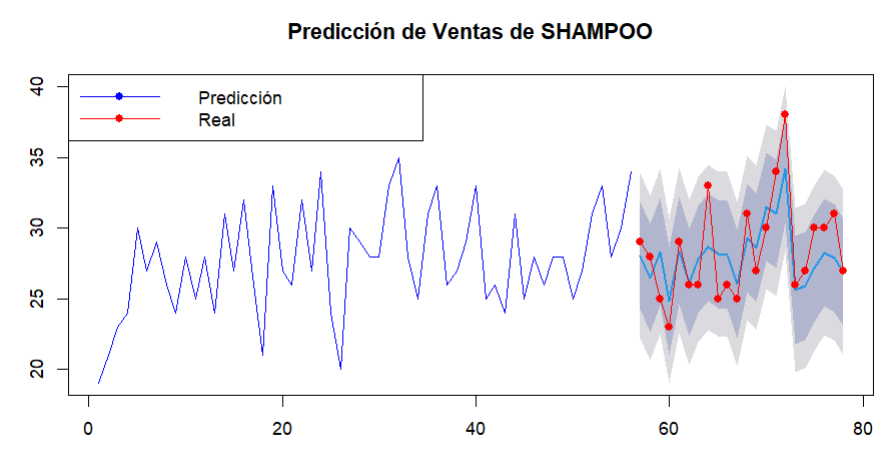
\includegraphics[width=0.8\textwidth]{i1.png}
\end{frame}
\begin{frame}{Visualizaci\'on: Predicci\'on vs. Real}
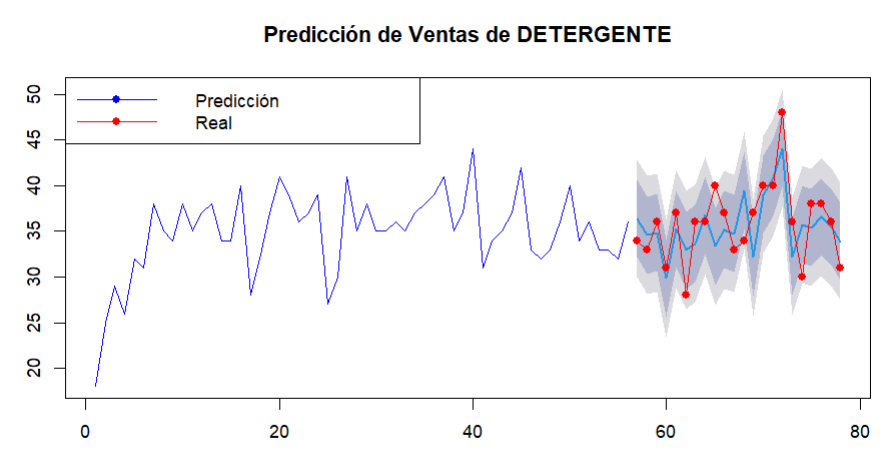
\includegraphics[width=0.8\textwidth]{i2.png}
\end{frame}
\begin{frame}{Visualizaci\'on: Predicci\'on vs. Real}
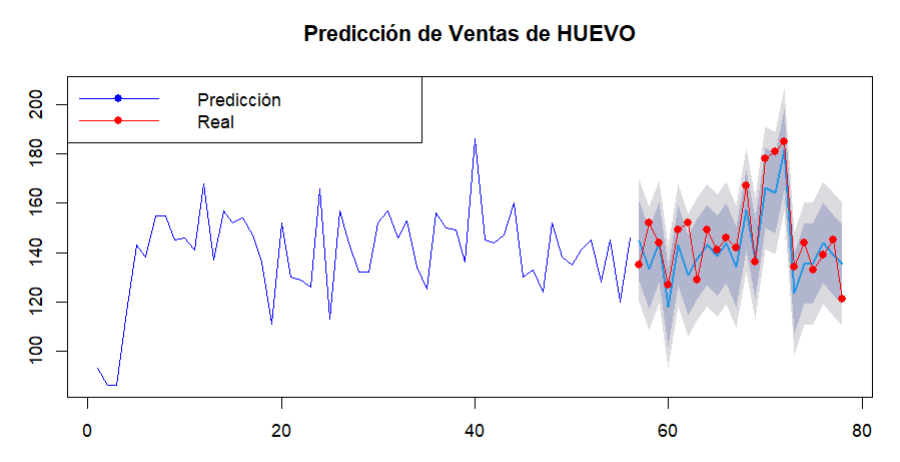
\includegraphics[width=0.8\textwidth]{i3.png}
\end{frame}
\begin{frame}{Visualizaci\'on: Predicci\'on vs. Real}
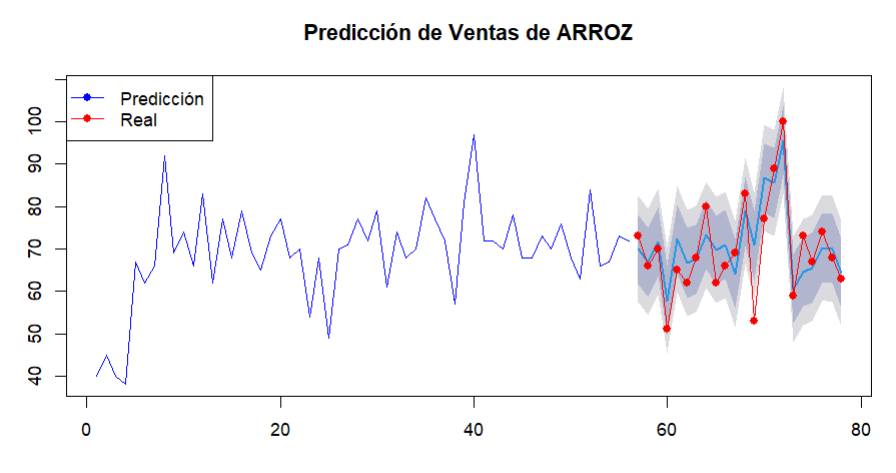
\includegraphics[width=0.8\textwidth]{i4.png}
\end{frame}
\begin{frame}{Visualizaci\'on: Predicci\'on vs. Real}
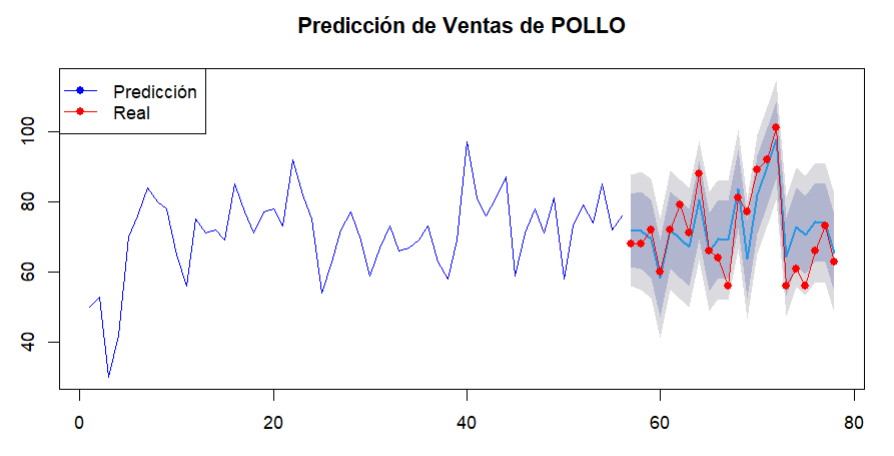
\includegraphics[width=0.8\textwidth]{i5.png}
\end{frame}
\begin{frame}{Visualizaci\'on: Predicci\'on vs. Real}
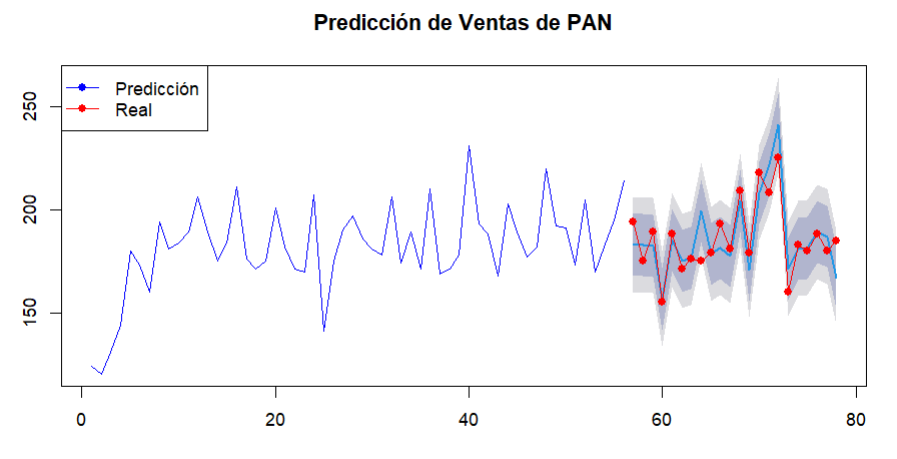
\includegraphics[width=0.8\textwidth]{i6.png}
\end{frame}
% --- Diapositiva 4: Optimizaci\'on de compras ---
\begin{frame}{Optimizaci\'on de decisiones de compra}
\begin{block}{Modelo de Programaci\'on Lineal Entera}
Maximiz\'o la ganancia semanal bajo:
\end{block}
\begin{itemize}
    \item Presupuesto m\'aximo: S/. 500 por semana
    \item L\'imite: no superar la demanda predicha
\end{itemize}
\vspace{0.3cm}
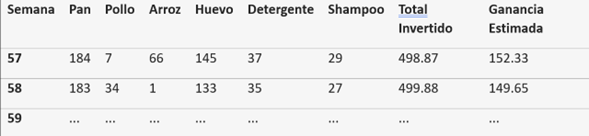
\includegraphics[width=0.75\textwidth]{tablaPRED.png}
\end{frame}

% --- Diapositiva 5: Inversi\'on y ganancia semanal ---
\begin{frame}{An\'alisis visual de los resultados}
\textbf{Inversi\'on y ganancia semanal (semanas 57--78)}
\begin{itemize}
    \item Inversi\'on cercana al l\'imite presupuestario
    \item Ganancia estable: > S/. 150, con picos hasta S/. 190
\end{itemize}
\vspace{0.3cm}
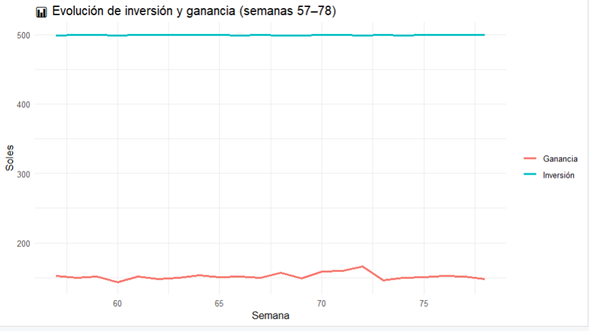
\includegraphics[width=0.75\textwidth]{Imagen3.png}
\end{frame}

% --- Diapositiva 6: Unidades adquiridas ---
\begin{frame}{Evoluci\'on de unidades adquiridas}
\begin{itemize}
    Prioriza lo rentable, reduce lo innecesario, y ajusta cada semana la compra según lo que más conviene
\end{itemize}
\vspace{0.3cm}
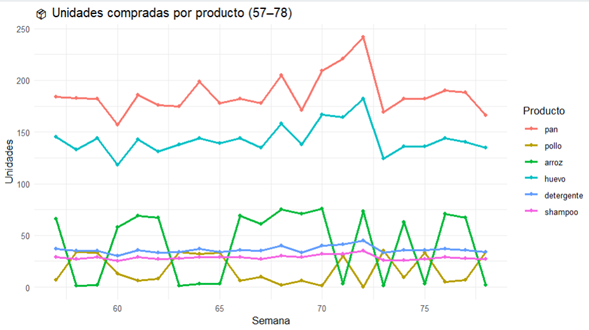
\includegraphics[width=0.8\textwidth]{uproducto1.png}
\end{frame}



\end{document}
